\documentclass[tikz]{standalone}
\usepackage{tikz,amsmath}
\begin{document}
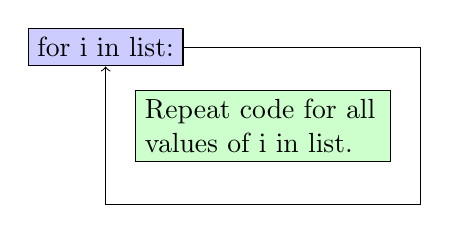
\begin{tikzpicture}
    \node (A) [rectangle, fill=blue!20, draw] at (0, 0) {for i in list:};
    \node [rectangle, fill=green!20, draw, text width=3cm] at (2, -1) {Repeat code for all values of i in list.};
    \draw [->] (A) -- (4,0) -- (4,-2) -- (0,-2) -- (A); 
\end{tikzpicture}
\end{document}
